\documentclass{article}
\usepackage[utf8]{inputenc}
\usepackage{authblk}
\usepackage{setspace}
\usepackage[margin=1.25in]{geometry}
\usepackage{graphicx}
\usepackage{xcolor}
\usepackage{float}
\graphicspath{ {./figures/} }
\usepackage{amsmath,amssymb,amsfonts}
\usepackage{booktabs}
\usepackage{natbib}
\usepackage{hyperref}
\hypersetup{colorlinks=true, linkcolor=blue, citecolor=blue, urlcolor=blue}

\title{\textbf{Does the Slope of the US Yield Curve Predict Six-Month-Ahead US Equity Returns? A Predictive Regression with Overlap-Robust Inference}}
\author[1]{SIQuant Research}
\affil[1]{Hypothesis $\times$ Quant}
\date{\today}
\onehalfspacing

\begin{document}
\maketitle

\begin{abstract}
\noindent \textbf{Hypothesis:} $H_0$: the 10y--3m spread has no predictive power for 126-session-ahead S\&P 500 returns; $H_1$: the slope coefficient is positive \\
\textbf{Data:} 2,387 daily observations, 2016-10-24 to 2026-04-24; 614 sessions with an inverted curve \\
\textbf{Method:} OLS with Newey--West HAC errors (126 lags) and a 2,000-draw circular-shift placebo; ACCEPTED only if both one-sided $p<0.05$ \\
\textbf{Results:} $\beta=-0.0262$ (HAC $t=-1.82$, $p=0.9659$; placebo $p=0.9250$), $R^2=0.074$.  \\
\textbf{Research decision:} \colorbox[rgb]{0.75,0.15,0.15}{\textcolor{white}{\textbf{\,REJECTED\,}}}
\end{abstract}

\section{Design}
The regressor is the 10-year minus 3-month Treasury spread observed at the close of day $t$; the outcome is the log return of the S\&P 500 from the close of $t$ to the close of $t+126$, so there is no look-ahead \citep{estrella1998predicting}. Overlapping outcomes induce strong serial correlation, therefore HAC errors with a lag equal to the horizon are used and a circular-shift placebo provides a non-parametric reference distribution for the $t$-statistic.

\section{Results}
Mean forward return is 8.33\% after inverted-curve sessions (614 sessions) and 5.63\% otherwise.

\begin{figure}[H]
\centering
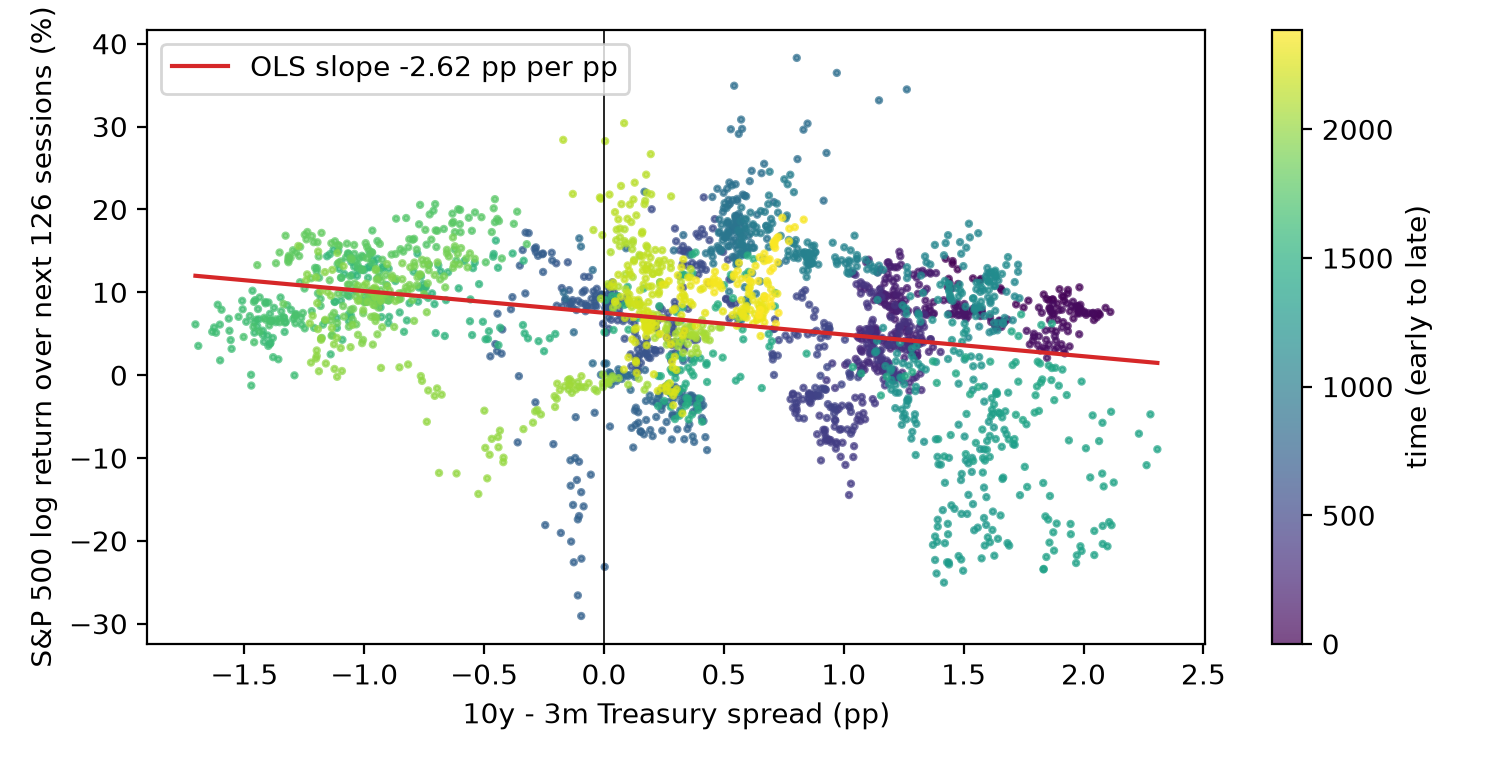
\includegraphics[width=0.8\textwidth]{fig1_spread_vs_forward_return.png}
\caption{Six-month-ahead S\&P 500 log return against the 10y--3m spread.}
\end{figure}

\section{Limitations}
The sample covers one full cycle with only two inversion episodes, so the effective number of independent observations is far smaller than the number of rows; the placebo accounts for this only partly. The spread is a market series and is not revised.


\bibliographystyle{plainnat}
\bibliography{references}

\end{document}
